\chapter{Конструкторский раздел}
\label{cha:design}

  \section{Разработка алгоритма}
  
    \subsection{Обоснование необходимости разработки алгоритма}
    
      Рассмотренные в аналитической части алгоритмы не поддерживают отображение дисперсионной картины на поверхностях прозрачных объетов, поэтому необходимо провести модификацию алгоритма для решения поставленной задачи. Для модификации был выбран алгоритм обратной трассировки лучей, так как он имеет физическую природу и поддерживает преломление лучей.

      Рассмотрим дисперсию с физической точки зрения.
    
    \subsection{Основные физические соотношения для дисперсии}
    
      Дисперсия света обусловлена зависимостью показателей преломления света от длины волны. Закон Снеллиуса (также Снелля или Снелла) описывает преломление света на границе двух прозрачных сред.

      Угол падения света на поверхность связан с углом преломления соотношением:

      \begin{equation}
         n_{1} sin(\theta_{1}) = n_{2} sin(\theta_{2}) 
      \end{equation}
      
      где $n_{1}$ — показатель преломления среды, из которой свет падает на границу раздела;
      
      $\theta_{1}$ — угол падения света — угол между падающим на поверхность лучом и нормалью к поверхности;
      
      $n_{2}$ — показатель преломления среды, в которую свет попадает, пройдя границу раздела;
      
      $\theta_{2}$ — угол преломления света — угол между прошедшим через поверхность лучом и нормалью к поверхности.
    
    \subsection{Описание алгоритма}
    
      Картина с дисперсией света может быть представлена на основании той же идеи что лежит в основе алгоритма обратной трассировки лучей: отслеживание луча света от глаз наблюдателя (камеры) и определение цветf пикселя на основании последовательных отражений от непрозрачных поверхностей и прохождений света сквозь прозрачные объекты. Новым фактором, который следуем учитывать в алгоритме, является разложение света на монохроматические лучи при преломлении.

      Проведем в алгоритме обратной трассировки следующие модификации:

      \begin{itemize}
        \item прозрачные объекты сцены должны также содержать коэффициент преломления света.
        \item в алгоритме стандартном трассировки лучей луч содержит геометрическую информацию, такую как начальную точки и направление. Добавим в алгоритм также флаг, определяющий является ли луч монохроматическим. Будет устанавливать этот флаг преломлении луча и разложении его на монохроматические лучи.
        \item Луч света раскладывается на 3 монохроматических луча: красный, зеленый, синий. После получений информации по каждому из них - цвета смешиваются.
        \item При пересечении прозрачной поверхности монохроматическим лучом, разложения луча происходить не должно.
      \end{itemize}
      
      \begin{figure}[h]
        \centering
        
        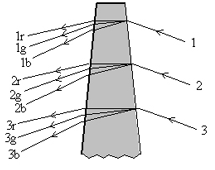
\includegraphics{images/light_decomposition.png}
        \caption{Разложение света на лучи при прохождении через програзный объект}
      \end{figure}

    \subsection{Описание структур данных}
    
      \begin{lstlisting}[caption=Структура луча]
struct ray {
  point point_start,
  vector ray_dir,
  bool is_monochrom,
  color
};
      \end{lstlisting}